%----------------------------------------------------------------------------------------
% Beamer Presentation
% LaTeX Template
% Version 1.0 (10/11/12)
%
% This template has been downloaded from:
% http://www.LaTeXTemplates.com
%
% License:
% CC BY-NC-SA 3.0 (http://creativecommons.org/licenses/by-nc-sa/3.0/)
%
% Modified by Laith Sahawneh / Randy Beard on July 27, 2013. C-UAS Style
%----------------------------------------------------------------------------------------
%	PACKAGES AND THEMES
%----------------------------------------------------------------------------------------
\documentclass{beamer}
\usetheme{Magicc}
\mode<presentation>

% Packages:
\usepackage{graphicx}                   		% Allows including images
\usepackage{booktabs}                   	% Allows the use of \toprule, \midrule and \bottomrule in tables
\usepackage{multimedia} 			% Allows movies to be embeded
\usepackage{algorithmic,algorithm}		% Package to include algorithms
	\algsetup{linenosize=\small}
\usepackage{textpos} 				% for positioning the C-UAS logo
\usepackage{tikz} 					% used to draw line under title


% Custom commands:
\newcommand{\abs}[1]{\left|{#1}\right|}
\newcommand{\norm}[1]{\left\|{#1}\right\|}

%--------------------------------- Document ---------------------------------------------
\begin{document}

%----------------------------------------------------------------------------------------
%	TITLE PAGE
%----------------------------------------------------------------------------------------
% The short title appears at the bottom of every slide, the full title is only on the title page:

\title[Short Title]{My Title} 
                                                                                   
\author[Short Name]{My Name} 

\institute[Short Institution]{
	Magicc Lab \\
	Brigham Young University \\
	\textit{myemail@byu.edu}
	}

%\date{\today} 
\date[]{}      % no date

% create the title page
{
%  \setbeamertemplate{footline}{}
%  \setbeamertemplate{headline}{}
%\setbeamercolor{background canvas}{bg=BYUblue!30}
\setbeamercolor{headline}{bg=BYUblue!20}
\setbeamertemplate{title page}[default][colsep=-4bp,rounded=true] % remove shadow on title page
  \begin{frame}
	\setbeamercolor{frame}{bg=BYUblue!50,fg=white!25}
%    \centering \includegraphics[width = 1.0in]{figures/magiccLabLogo} 
%    \raggedleft \includegraphics[width = 1.0in]{figures/magiccLabLogo} 
    \vspace{1cm}
    \titlepage  
  \end{frame}
%\setbeamercolor{background canvas}{bg=}
}

%----------------------------------------------------------------------------------------
%	OUTLINE
%----------------------------------------------------------------------------------------

\setbeamertemplate{section in toc}[ball unnumbered]
\setbeamertemplate{subsection in toc}[ball unnumbered]

% Outline slide (created from \section{} and \subsection{}
\begin{frame}
	\frametitle{Outline} 
	\tableofcontents     
\end{frame}

%----------------------------------------------------------------------------------------
%	PRESENTATION SLIDES
%----------------------------------------------------------------------------------------

%------------------------------------------------
\section{Motivation} % for the outline
%------------------------------------------------

%\subsection*{Motivation1} % can also include subsections for outline

\begin{frame}
	\frametitle{Motivational Slide}
%	\centering
%	\begin{center}
%		\movie[height=3in,width=4in,poster]{}{Videos/}
%	\end{center}
	% Consider using movie15 package to trime first 10 seconds... ect.
\end{frame}

%------------------------------------------------
\section{Cool Results} % for the outline
%------------------------------------------------

%\subsection*{Motivation1} % can also include subsections for outline

% add outline page with current section highlighted.
\begin{frame}
	\frametitle{Outline}
	\tableofcontents[currentsection]
	%\tableofcontents[currentsection,currentsubsection]
\end{frame}

\begin{frame}
	\frametitle{Results Slide}
%	\centering
%	\begin{center}
%		\movie[height=3in,width=4in,poster]{}{Videos/}
%	\end{center}
	% Consider using movie15 package to trime first 10 seconds... ect.
\end{frame}


%------------------------------------------------
\section{Conclusions}  % for the outline

% add outline page with current section highlighted.
\begin{frame}
	\frametitle{Outline}
	\tableofcontents[currentsection]
	%\tableofcontents[currentsection,currentsubsection]
\end{frame}

\begin{frame}
	\frametitle{Conclusions}
%	\centering
%	\begin{center}
%		\movie[height=3in,width=4in,poster]{}{Videos/}
%	\end{center}
	% Consider using movie15 package to trime first 10 seconds... ect.
\end{frame}


\end{document}
%---------------------------------------  End --------------------------------------------

%% EXAMPLE OF HOW TO DO BLOCKS--DIEFFERNT THAN THEOREMS???
%\begin{frame}
%\frametitle{Blocks of Highlighted Text}
%\begin{block}{Block Title}
%Stuff Here
%\end{block}

% EXAMPLE OF HOW TO DO MULTI COLUMNS
%\begin{frame}
%\frametitle{Multiple Columns}
%\begin{columns}[c] % The "c" option specifies centered vertical alignment while the "t" option is used for top vertical alignment
%\column{.45\textwidth} % Left column and width
%\textbf{Heading}
%\begin{enumerate}
%\item Statement
%\item Explanation
%\item Example
%\end{enumerate}

%\column{.5\textwidth} % Right column and width
%Lorem ipsum dolor sit amet, consectetur adipiscing elit. Integer lectus nisl, ultricies in feugiat rutrum, porttitor sit amet augue. Aliquam ut tortor mauris. Sed volutpat ante purus, quis accumsan dolor.

%\end{columns}
%\end{frame}


%% EXAMPLE OF HOW TO DO A TABLE
%\begin{frame}
%\frametitle{Table}
%\begin{table}
%\begin{tabular}{l l l}
%\toprule
%\textbf{Treatments} & \textbf{Response 1} & \textbf{Response 2}\\
%\midrule
%Treatment 1 & 0.0003262 & 0.562 \\
%Treatment 2 & 0.0015681 & 0.910 \\
%Treatment 3 & 0.0009271 & 0.296 \\
%\bottomrule
%\end{tabular}
%\caption{Table caption}
%\end{table}
%\end{frame}

%------------------------------------------------

%% EXAMPLE OF HOW TO DO THEOREM BOXES
%\begin{frame}
%\frametitle{Theorem}
%\begin{theorem}[Mass--energy equivalence]
%$E = mc^2$
%\end{theorem}
%\end{frame}

%------------------------------------------------

%% EXAMPLE USING PSEUDO-CODE
%\begin{frame}[fragile] % Need to use the fragile option when verbatim is used in the slide
%\frametitle{Verbatim}
%\begin{example}[Theorem Slide Code]
%\begin{verbatim}
%\begin{frame}
%\frametitle{Theorem}
%\begin{theorem}[Mass--energy equivalence]
%$E = mc^2$
%\end{theorem}
%\end{frame}\end{verbatim}
%\end{example}
%\end{frame}

%------------------------------------------------

% EXAMPLE OF FIGURE 
%\begin{frame}
%\frametitle{Figure}
%%\begin{figure}
%%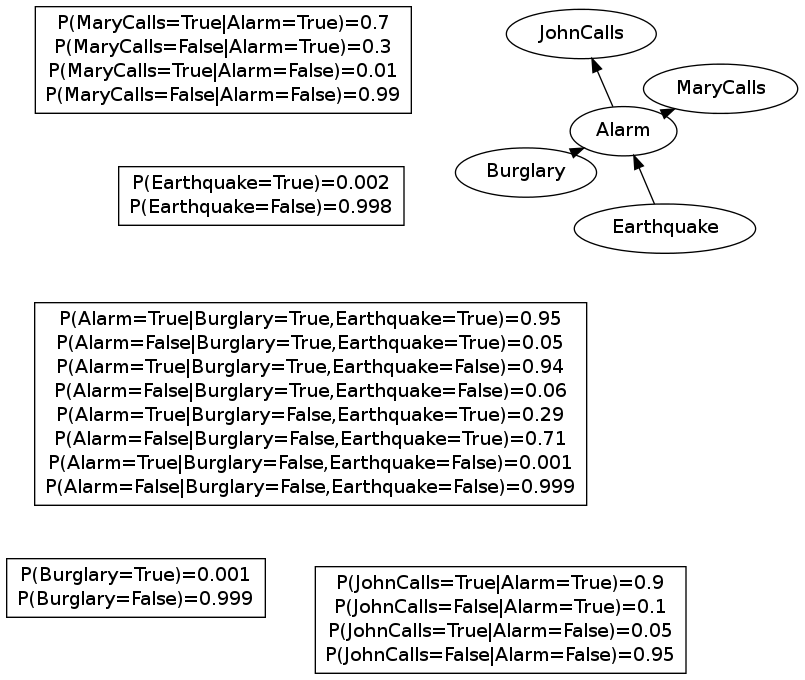
\includegraphics[width=0.8\linewidth]{figures/test}
%%\end{figure}
%\end{frame}

%------------------------------------------------


% EXAMPLE OF SLIDE WITH CITATION
%\begin{frame}[fragile] % Need to use the fragile option when verbatim is used in the slide
%\frametitle{Citation}
%An example of the \verb|\cite| command to cite within the presentation:\\~

%This statement requires citation \cite{p1}.
%\end{frame}

%------------------------------------------------

% EXAMPLE OF REFERENCE SLIDE
%\begin{frame}
%\frametitle{References}
%\footnotesize{
%\begin{thebibliography}{99} % Beamer does not support BibTeX so references must be inserted manually as below
%\bibitem[Smith, 2012]{p1} John Smith (2012)
%\newblock Title of the publication
%\newblock \emph{Journal Name} 12(3), 45 -- 678.
%\end{thebibliography}
%}
%\end{frame}

%----------------------------------------------------------------------------------------
